\documentclass[tikz]{standalone}

\begin{document}
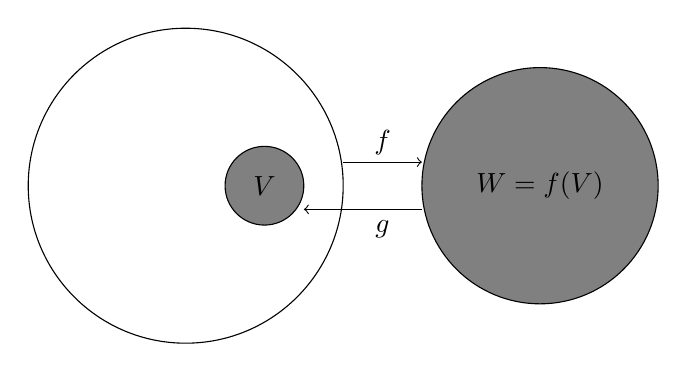
\begin{tikzpicture}
  \draw (-2, 0) circle (2);
  \draw[fill=gray] (2.5, 0) circle (1.5);
  \draw[fill=gray] (-1, 0) circle (0.5);
  \draw[->] (0, 0.3) -- (1, 0.3);
  \draw[->] (1, -0.3) -- (-0.5, -0.3);

  \node at (-1, 0) {$V$};
  \node at (2.5, 0) {$W = f(V)$};

  \node at (0.5, 0.55) {$f$};
  \node at (0.5, -0.55) {$g$};
\end{tikzpicture}
\end{document}
